\section{Funkcionális követelmények}

A funkcionális követelmények azt határozzák meg, hogy a rendszernek milyen konkrét műveleteket kell támogatnia a felhasználók és az alkalmazás szempontjából. A WatchDB esetében ezek a követelmények közvetlenül a termékkoncepcióból és az MVP-ben meghatározott funkciókból vezethetőek le: a felhasználónak tudnia kell fiókot létrehozni, filmeket keresni, filmeket listába menteni, megnézett filmeket naplózni, értékelést adni, valamint saját profiloldalán áttekinteni az összegyűjtött adatokat.

\begin{figure}[H]
\centering
\small
\begin{tikzpicture}[
    node distance=0.62cm and 0.95cm,
    appnode/.style={
        draw,
        rounded corners,
        fill=blue!8,
        align=center,
        text width=2.8cm,
        minimum height=1cm,
        font=\bfseries
    },
    modulenode/.style={
        draw,
        rounded corners,
        fill=gray!8,
        align=center,
        text width=3.2cm,
        minimum height=0.82cm
    },
    modulearrow/.style={-{Latex[length=2mm]}, thick}
]
\node[appnode] (watchdb) {WatchDB};
\node[modulenode, above=of watchdb] (auth) {Autentikáció};
\node[modulenode, left=of watchdb] (search) {Filmkeresés};
\node[modulenode, right=of watchdb] (details) {Filmrészletek};
\node[modulenode, below left=of watchdb] (watchlist) {Watchlist};
\node[modulenode, below=of watchdb] (watched) {Watched log\\és rating};
\node[modulenode, below right=of watchdb] (profile) {Profiloldal};

\draw[modulearrow] (watchdb) -- (auth);
\draw[modulearrow] (watchdb) -- (search);
\draw[modulearrow] (watchdb) -- (details);
\draw[modulearrow] (watchdb) -- (watchlist);
\draw[modulearrow] (watchdb) -- (watched);
\draw[modulearrow] (watchdb) -- (profile);
\end{tikzpicture}
\caption{A WatchDB fő funkcionális egységei}
\label{fig:watchdb-functional-modules}
\end{figure}

Az alkalmazás első alapvető funkciója az autentikáció. A rendszernek támogatnia kell az új felhasználók regisztrációját, a meglévő felhasználók bejelentkezését és kijelentkezését, valamint a munkamenet kezelését. Mivel a watchlist és a megnézett filmek listája felhasználóhoz kötött adat, ezek a műveletek csak bejelentkezett állapotban végezhetők el. Amennyiben egy nem autentikált látogató olyan műveletet próbál végrehajtani, amely felhasználói fiókot igényel, az alkalmazásnak jeleznie kell, hogy a folytatáshoz bejelentkezés vagy regisztráció szükséges.

A filmkeresés a rendszer egyik központi funkciója. A felhasználónak lehetőséget kell kapnia arra, hogy cím alapján filmeket keressen, majd a találatok között megtekinthesse az alapvető információkat, például a film címét, poszterét, megjelenési évét és rövid leírását. A keresési funkció külső filmes adatforrásra épül, ezért az alkalmazásnak a keresési kéréseket úgy kell továbbítania, hogy a felhasználó számára a válasz gyorsan és áttekinthető formában jelenjen meg. A keresési eredményekből a felhasználó tovább tud lépni az adott film részletes oldalára.

\begin{figure}[H]
\centering
\scriptsize
\begin{tikzpicture}[
    actor/.style={
        draw,
        rounded corners,
        fill=gray!8,
        align=center,
        minimum height=0.62cm,
        text width=2.35cm
    },
    message/.style={-{Latex[length=2mm]}, thick},
    returnmessage/.style={-{Latex[length=2mm]}, thick, dashed},
    lifeline/.style={gray, dashed}
]
\node[actor] (user) at (0,0.5) {Felhasználó};
\node[actor] (ui) at (3.2,0.5) {WatchDB felület};
\node[actor] (api) at (6.45,0.5) {Next.js API route};
\node[actor] (tmdb) at (9.7,0.5) {TMDB API};

\draw[lifeline] (0,0.2) -- (0,-6.6);
\draw[lifeline] (3.2,0.2) -- (3.2,-6.6);
\draw[lifeline] (6.45,0.2) -- (6.45,-6.6);
\draw[lifeline] (9.7,0.2) -- (9.7,-6.6);

\draw[fill=white] (3.08,-0.95) rectangle (3.32,-5.95);
\draw[fill=white] (6.33,-1.75) rectangle (6.57,-5.2);
\draw[fill=white] (9.58,-2.55) rectangle (9.82,-4.3);

\draw[message] (0,-1.15) -- node[above, align=center] {keresési kifejezés\\megadása} (3.08,-1.15);
\draw[message] (3.32,-1.95) -- node[above, align=center] {\texttt{GET /api/search}\\query paraméterrel} (6.33,-1.95);
\draw[message] (6.57,-2.75) -- node[above, align=center] {keresés továbbítása} (9.58,-2.75);
\draw[returnmessage] (9.58,-3.75) -- node[above, align=center] {találatok\\visszaadása} (6.57,-3.75);
\draw[returnmessage] (6.33,-4.55) -- node[above, align=center] {normalizált\\válasz} (3.32,-4.55);
\draw[message] (3.08,-5.35) -- node[above, align=center] {eredmények\\megjelenítése} (0,-5.35);
\end{tikzpicture}
\caption{A filmkeresés fő adatáramlása}
\label{fig:watchdb-search-flow}
\end{figure}

A filmrészletek oldalon a rendszernek részletesebb információkat kell megjelenítenie az adott filmről. Ide tartozhat a cím, a poszter, a háttérkép, a megjelenési dátum, a játékidő, a műfajok, az eredeti nyelv, a rövid tartalmi leírás és a külső adatforrásból származó értékelési információ. Ez az oldal szolgál kiindulópontként a felhasználói műveletekhez is, például a watchlisthez adáshoz vagy a film megnézettként való megjelöléséhez.

A watchlist funkció célja, hogy a felhasználó el tudja menteni azokat a filmeket, amelyeket később szeretne megnézni. A rendszernek biztosítania kell egy film hozzáadását a watchlisthez, a film eltávolítását a listából, valamint a teljes watchlist megjelenítését a profiloldalon. Fontos követelmény, hogy egy adott film státusza egyértelmű legyen a felhasználó számára: ha a film már szerepel a watchlisten, akkor a felületnek ezt jeleznie kell, és a műveletnek eltávolításként kell viselkednie.

\begin{figure}[H]
\centering
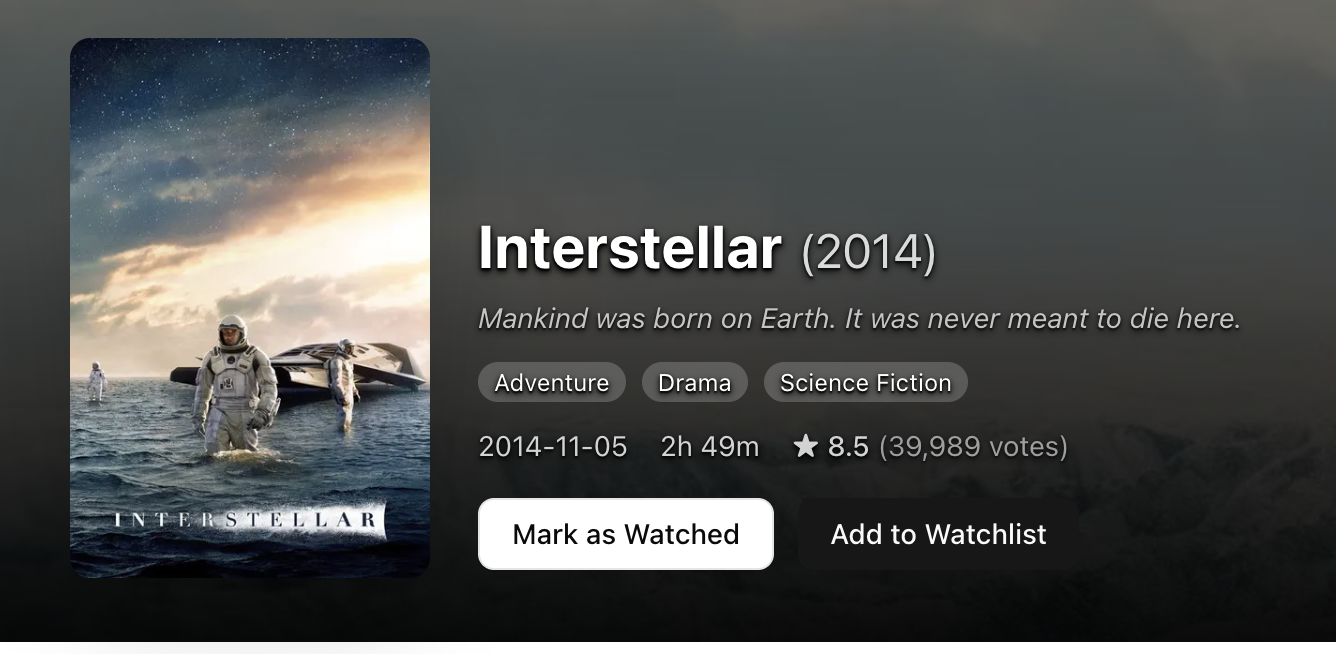
\includegraphics[width=0.82\textwidth]{chapters/chapter-5-systemSpecs/mark-as-watched.png}
\vspace{0.5em}

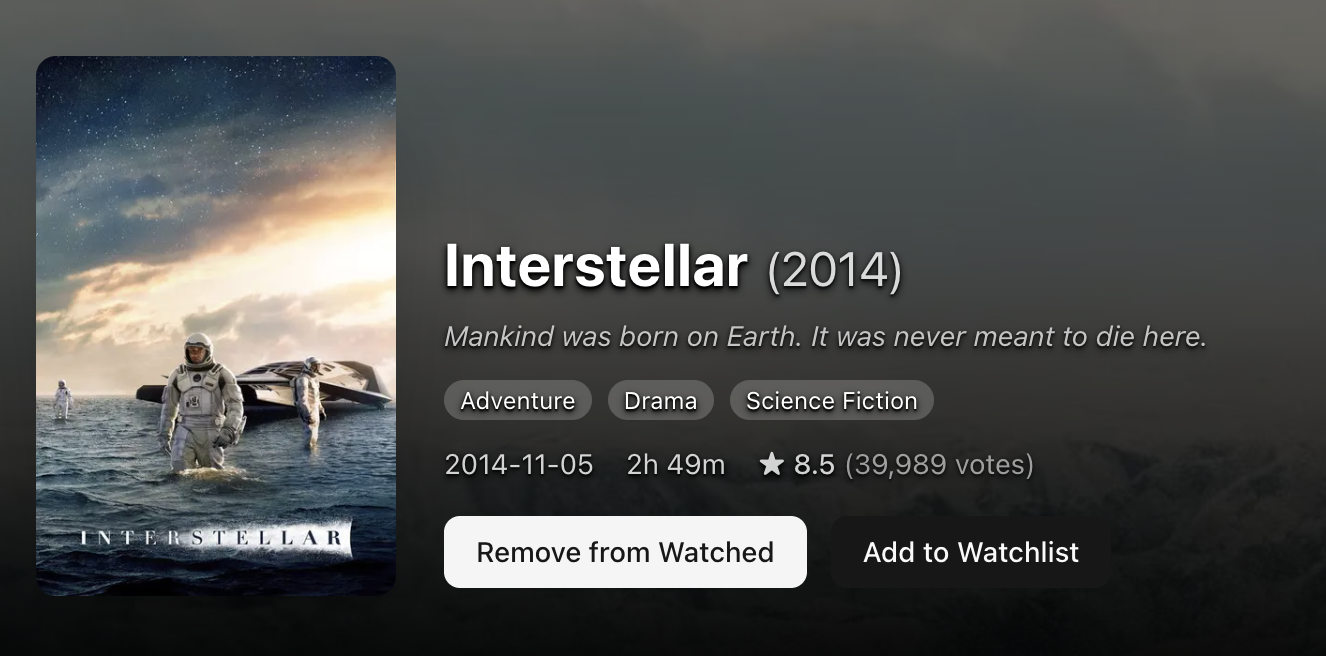
\includegraphics[width=0.82\textwidth]{chapters/chapter-5-systemSpecs/remove-from-watched.png}
\caption{A megnézettként jelölés állapotváltozása a filmrészletek oldalon}
\label{fig:watchdb-mark-watched-state}
\end{figure}

A megnézett filmek naplózása a WatchDB másik alapfunkciója. A felhasználónak meg kell tudnia jelölni egy filmet megnézettként, meg kell tudnia adni hozzá egy személyes értékelést, valamint opcionálisan a megtekintés dátumát. A személyes értékelés 1 és 5 közötti értéket vehet fel, amely a profiloldalon is megjelenik. Amikor egy film megnézettként kerül naplózásra, a rendszernek kezelnie kell azt az esetet is, ha a film korábban watchlisten szerepelt, mivel ilyen esetben a film már nem egyszerűen tervezett, hanem teljesített megtekintésként értelmezhető.

A profiloldalnak összefoglaló nézetet kell adnia a felhasználó saját filmjeiről. Az MVP részeként a profil két fő listát jelenít meg: a megnézett filmeket és a watchlist elemeit. A megnézett filmeknél meg kell jelenjen a személyes értékelés, a naplózás vagy megtekintés dátuma, valamint a film alapvető vizuális adatai. A watchlist esetében a rendszernek azoknak a filmeknek a listáját kell megjelenítenie, amelyeket a felhasználó későbbi megtekintésre mentett el.

Összefoglalva, a funkcionális követelmények a WatchDB MVP működésének magját írják le. Ezek biztosítják, hogy az alkalmazás ne csupán filmes információkat jelenítsen meg, hanem személyes filmnaplóként is használható legyen. A későbbi verziókban erre az alapra épülhetnek rá a közösségi funkciók, például a publikus profilok, követési rendszer, aktivitási feed vagy ajánlási mechanizmusok.
